\pagestyle{empty}
\renewcommand{\headrulewidth}{0pt}
\renewcommand{\footrulewidth}{0pt}
\lhead{}\chead{}\rhead{}
\lfoot{}\cfoot{\thepage}\rfoot{}

\newcommand{\HeaderLineSpace}{-0.25cm}
\newcommand{\UniTextRO}{UNIVERSITATEA POLITEHNICA DIN BUCUREȘTI \\[\HeaderLineSpace]
FACULTATEA DE AUTOMATICĂ ȘI CALCULATOARE \\[\HeaderLineSpace]
DEPARTAMENTUL DE CALCULATOARE\\}
\newcommand{\DiplomaRO}{PROIECT DE DIPLOMĂ}
\newcommand{\AdvisorRO}{Coordonatori științifici:}
\newcommand{\BucRO}{BUCUREȘTI}

\newcommand{\UniTextEN}{UNIVERSITY POLITEHNICA OF BUCHAREST \\[\HeaderLineSpace]
FACULTY OF AUTOMATIC CONTROL AND COMPUTERS \\[\HeaderLineSpace]
COMPUTER SCIENCE AND ENGINEERING DEPARTMENT\\}
\newcommand{\DiplomaEN}{DIPLOMA PROJECT}
\newcommand{\AdvisorEN}{Thesis advisors:}
\newcommand{\BucEN}{BUCHAREST}

\newcommand{\frontPage}[6]{
\begin{titlepage}
\begin{center}
{\Large #1}  % header (university, faculty, department)
\vspace{50pt}
\begin{tabular}{p{6cm}p{4cm}}

\includegraphics[scale=0.8]{pics/upb-logo.jpg} &
	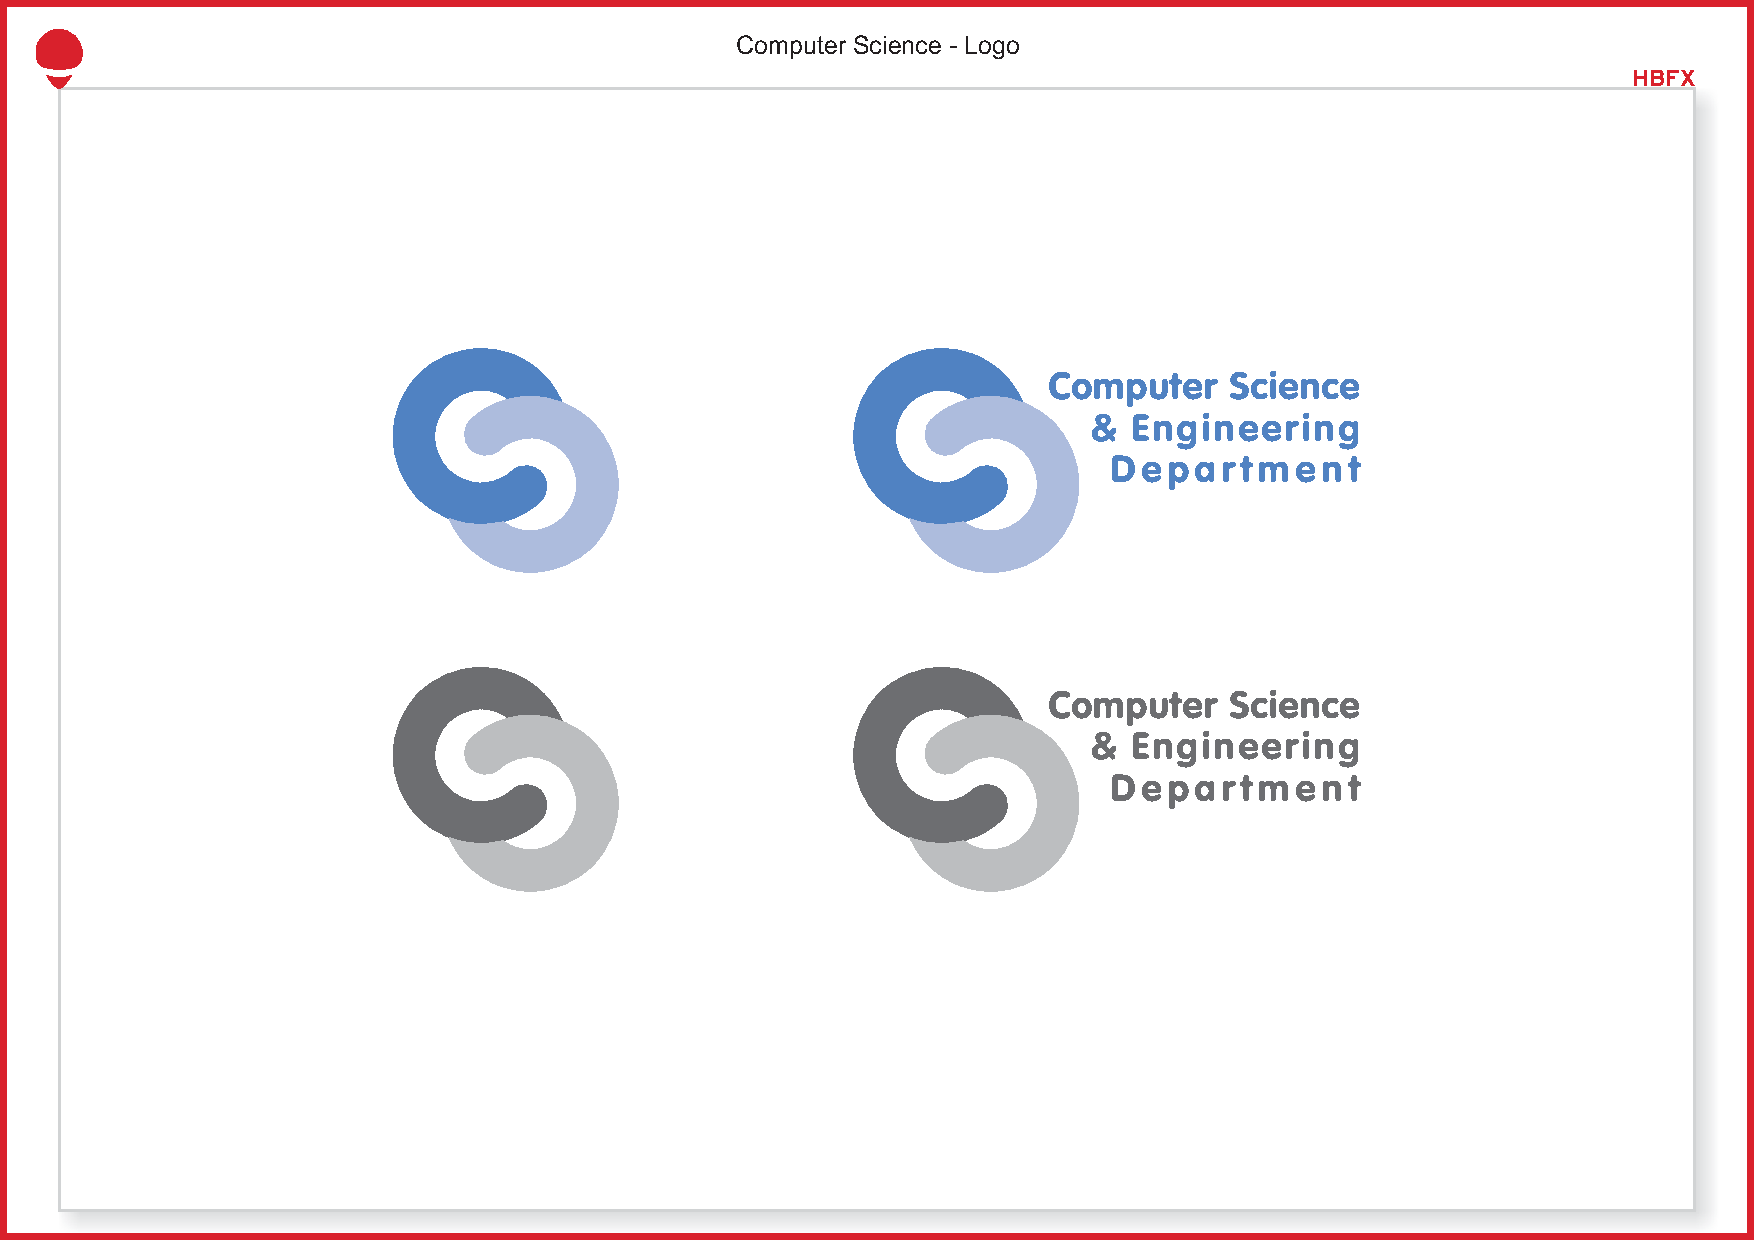
\includegraphics[scale=0.5,trim={14cm 11cm 2cm 5cm},clip=true]{pics/cs-logo.pdf}
\end{tabular}

\vspace{105pt}
{\Huge #2}\\                           % diploma project text
\vspace{40pt}
{\Large #3}\\ \vspace{0pt}  % project title
{\Large #4}\\                          % project subtitle
\vspace{40pt}
{\LARGE \Name}\\                   % student name
\end{center}
\vspace{60pt}
\begin{tabular*}{\textwidth}{@{\extracolsep{\fill}}p{6cm}r}
&{\large\textbf{#5}}\vspace{10pt}\\      % scientific advisor
&{\large \Advisor}\\                     % first advisor
&{\large \AdvisorTwo}                    % second advisor
\end{tabular*}
\vspace{20pt}
\begin{center}
{\large\textbf{#6}}\\                                % bucharest
\vspace{0pt}
{\normalsize \Year}
\end{center}
\end{titlepage}
}

\newcommand{\frontPageRO}{\frontPage{\UniTextRO}{\DiplomaRO}{\ProjectTitleRO}{\ProjectSubtitleRO}{\AdvisorRO}{\BucRO}}
\newcommand{\frontPageEN}{\frontPage{\UniTextEN}{\DiplomaEN}{\ProjectTitleEN}{\ProjectSubtitleEN}{\AdvisorEN}{\BucEN}}

\linespread{1.15}
\setlength\parindent{0pt}
\setlength\parskip{.28cm}

%% Abstract macro
\newcommand{\AbstractPage}{
\begin{titlepage}
\textbf{\large SINOPSIS}\par
\AbstractRO\par\vfill
\textbf{\large ABSTRACT}\par
\AbstractEN \vfill
\end{titlepage}
}

%% Thank you macro
\newcommand{\ThanksPage}{
\begin{titlepage}
{\noindent \large\textbf{MULȚUMIRI}}\\
\Thanks
\end{titlepage}
}

%%% Puteți elimina aceste linii din lucrare, servesc numai pentru template.
\newcommand{\worktype}[1]{[\textit{#1}] }
\newcommand{\dezvoltare}{\worktype{Dezvoltare de produs}}
\newcommand{\cercetare}{\worktype{Cercetare}}
\newcommand{\ambele}{\worktype{Ambele}}
%%%

%%
%%   Campurile de mai jos trebuie modificate de autor. Modificati doar continutul, nu si numele fiecarei definitii
%%
\newcommand{\ProjectTitleRO}{Studiu de Caz al Evaluarii Costurilor de Portare:
Portarea IxOS pe placute ARM}
\newcommand{\ProjectSubtitleRO}{~ }
\newcommand{\ProjectTitleEN}{Case Study of Evaluating Porting Costs: Porting IxOS on ARM Boards}
\newcommand{\ProjectSubtitleEN}{~ }
\newcommand{\Name}{Lucian-Ioan Popescu}
\newcommand{\Advisor}{Dr. ing. Lucian Mogosanu}
\newcommand{\AdvisorTwo}{Conf. Dr. ing. Razvan Deaconescu}
\newcommand{\Year}{2022}

\newcommand\todo[1]{\textcolor{red}{#1}}
\newcommand{\lm}[1]{\textcolor{blue}{\bf [LM: #1]}}
\newcommand{\lp}[1]{\textcolor{red}{\bf [LP: #1]}}
